\section{IRT for Leaderboards}
\label{ch:isicle:exp}

Leaderboards should: (1) reliably and efficiently rank
better models ahead of worse
models~\citep{sutcliffe1992pragmatics,voorhees2003evaluating} and (2)
guide inspection of \itms{} and \subjs{} (\S\ref{ch:isicle:interp}).
%
The first ameliorates the unavoidable randomness
of finite evaluations while the second enables
error analysis~\citep{wu2019errudite} and model
probing~\citep{belinkov2019survey,zhang2019manifold}.
%
First we verify that \irt{} models accurately predict the \resps{} of
\subjs{} (\S\ref{ch:isicle:irt-accurate}).
%
Next, a ranking stability analysis shows that \irt{} has
modestly better reliability than classical rankings
(\S\ref{ch:isicle:irt-compare}).
%
Lastly, using \irt{} to actively sample \itms{} for annotation yields
rankings with better correlation to complete test data
(\S\ref{ch:isicle:sampling}).

\subsection{Why a Linear Model Baseline}

At first blush, the differences between \irt{} and logistic regression
are minimal, but we include the comparison to address natural
questions from the \abr{nlp} community:
%
(1) do the idiosyncrasies of the \irt{} formulation hurt
accuracy?
%
(2) should we add features to better understand phenomena
in the questions?
%
(3) why not use deep models?

The next section argues that both \irt{} and logistic regression are
accurate even without laboriously engineered task-specific features.
%
Adding obvious features such as \itm{} words (e.g., questions)
only minimally improves the accuracy.
%
We explicitly omit less interpretable deep models since our goal is to
make leaderboards \emph{more} interpretable.

\subsection{Response Prediction is Accurate}
\label{ch:isicle:irt-accurate}

Just as educational testing researchers validate \irt{} models by
seeing if they predict \subj{} \resps{}
correctly~\citep{aera2014standards}, we validate how well \name{} predicts
whether \squad{} models get questions right.

We compare against a logistic regression linear model (\abr{lm})
implemented with Vowpal Wabbit~\citep{Agarwal2014ARE}.
%
Since integrating hand-crafted features is easy, we incorporate
features derived from \subj{} \abr{id}s; \itm{} \abr{id}s; functions
of the \squad{} question, answer, and title; and \irt{} parameters
(details in Appendix~\ref{ch:isicle:apx:features}).
%
As in \irt{}, logistic regression predicts whether a \subj{} correctly
responds to an \itm{}.
%
Later, we discuss ways to integrate more features into \irt{}
(\S\ref{ch:isicle:future}).

\subsubsection{SQuAD Leaderboard Data}
\label{ch:isicle:datasets}
Experiments are on the \squad{} 2.0 leaderboard.
Development data are publicly available, and organizers provide test set responses.
There are $161$ development \subjs{}, $115$ test \subjs{}, and \num[group-separator={,}]{11873} \itms{} ($1.9$ million total pairs).
Experiments that do not need test responses use all development \subjs{}; those that do use the smaller test subset.

\subsubsection{Evaluation Scheme}

Following prior work~\citep{wu2020virt}, we evaluate \irt{} and linear models by holding out 10\% of responses and computing classification metrics.\footnote{Everywhere else in the paper, we train on all responses.}
%
In \squad{}, predicting whether a \resp{} is correct is an imbalanced
classification problem (80.4\% of responses in the development set are
correct).
%
Thus, we use \abr{roc auc}, macro F1, and accuracy.

\subsubsection{IRT Response Prediction is Accurate}
\label{ch:isicle:irt-compare}

\irt{} models that incorporate more priors into the generative story should be better, but are they?
We compare four \irt{} models: \pl{1}, \pl{2}, \pl{3}, and \pl{m}~(\S\ref{ch:isicle:lead}).
The more sophisticated models are better and all improve over the
\abr{lm} (Figure~\ref{fig:vw-ablation}) and correlate well with each other (Appendix~\ref{apx:irt-self-corr}).
To be clear, while higher accuracy than \abr{lm} is good, our goal is to validate that \irt{} models are accurate; later, we inspect model errors and identify annotation errors (\S\ref{ch:isicle:interp}).

\begin{figure*}[th]
    \centering
    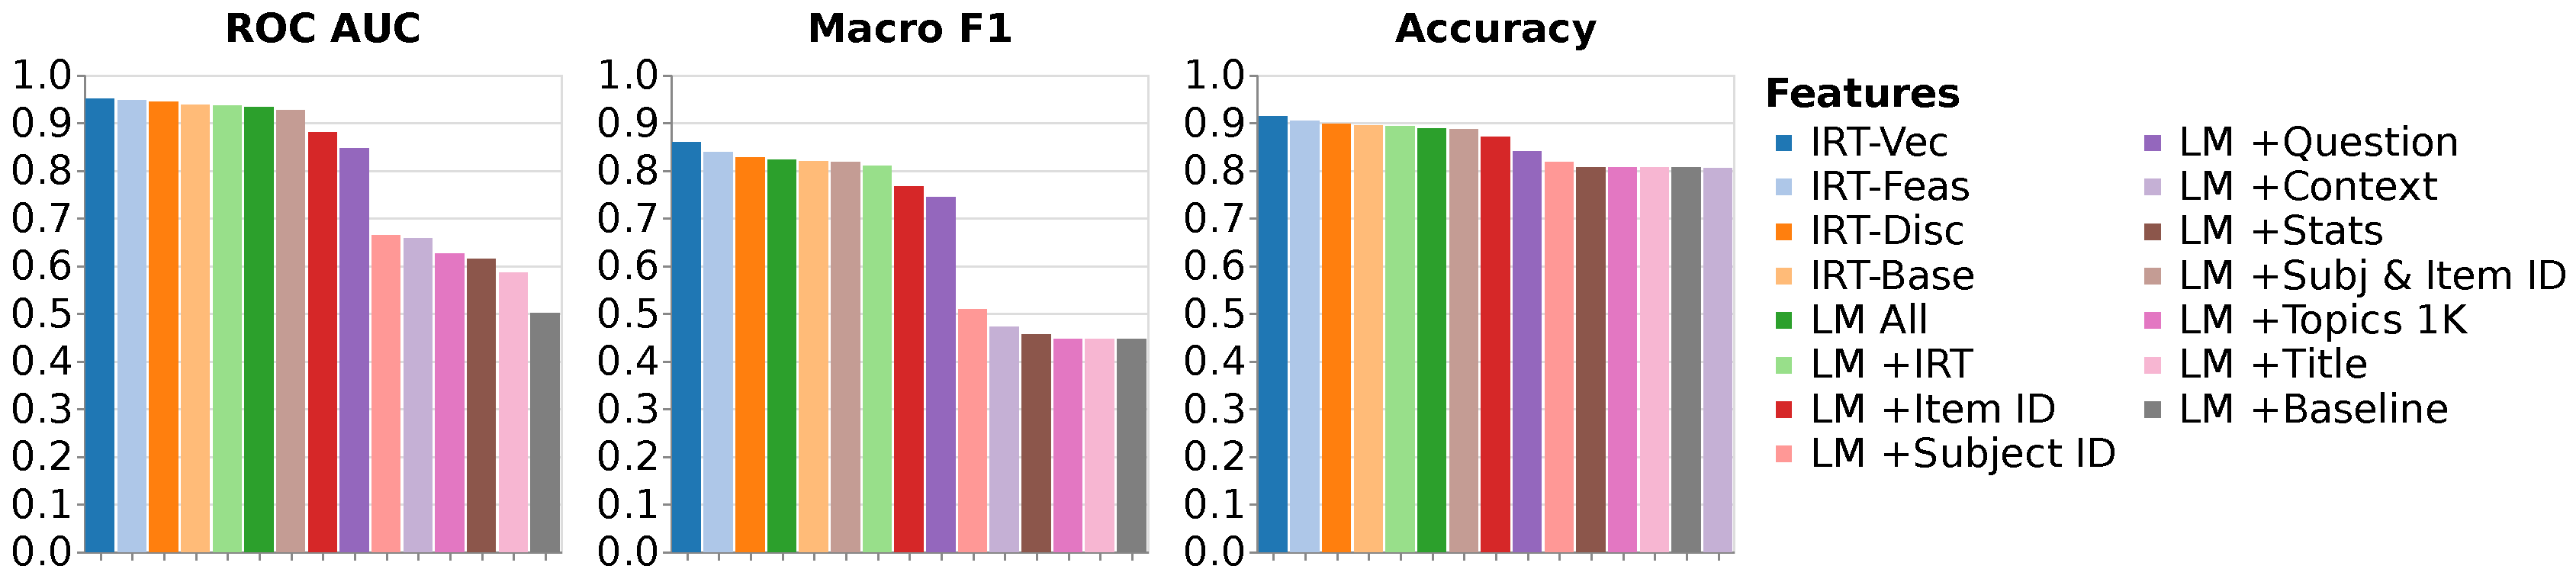
\includegraphics[width=\textwidth]{vw_ablation}
    \caption{
        We compare each \irt{} and linear model (\abr{lm}) by how well they predict \subj{} \resps{}.
        We focus on \abr{roc auc} since predicting responses is an imbalanced classification problem (most \subjs{} are correct).
        Under that metric, all \irt{} models improve over the best
        \abr{lm}, and the strongest \abr{lm} ablation only uses \irt{} features.
        That textual features are predictive in the \abr{lm} suggests they could improve future models.
    }
    \label{fig:vw-ablation}
\end{figure*}


\subsubsection{What Model Features are Predictive?}

Integrating additional features into Bayesian models is not trivial,
so we instead use the flexibility of linear models to identify useful
features.
%
Our leave-one-in ablation compares features (Figure~\ref{fig:vw-ablation}):
the top ablations both use \irt{} features, further validating
\irt{} parameters.
%
The \subj{} and \itm{} identifier features are also
strongly predictive, but \itm{} is the stronger of the two.
%
Text-based features are weaker, but this suggests future work to
better integrate them into \irt{} models (\S\ref{ch:isicle:future}).



\subsection{Ranking with IRT}

Leaderboards should produce \iemph{reliable} \subj{} rankings: can
\name{} rank systems even with a tiny test set?
%
Thus, we compare the correlation both of traditional average accuracy
(\S\ref{ch:isicle:agg}) and \irt{} rankings on the whole test
set compared to the rankings of the same metric on a smaller test set.
%
Our first experiment (\S\ref{ch:isicle:stable}) examines the stability
of existing \itms{} and \subjs{} while the second
(\S\ref{ch:isicle:sampling}) investigates stability of ``new''
evaluation data using sampling strategies.

\subsubsection{IRT Rankings Have Better Reliability}
\label{ch:isicle:stable}

\begin{figure*}[t]
    \centering
    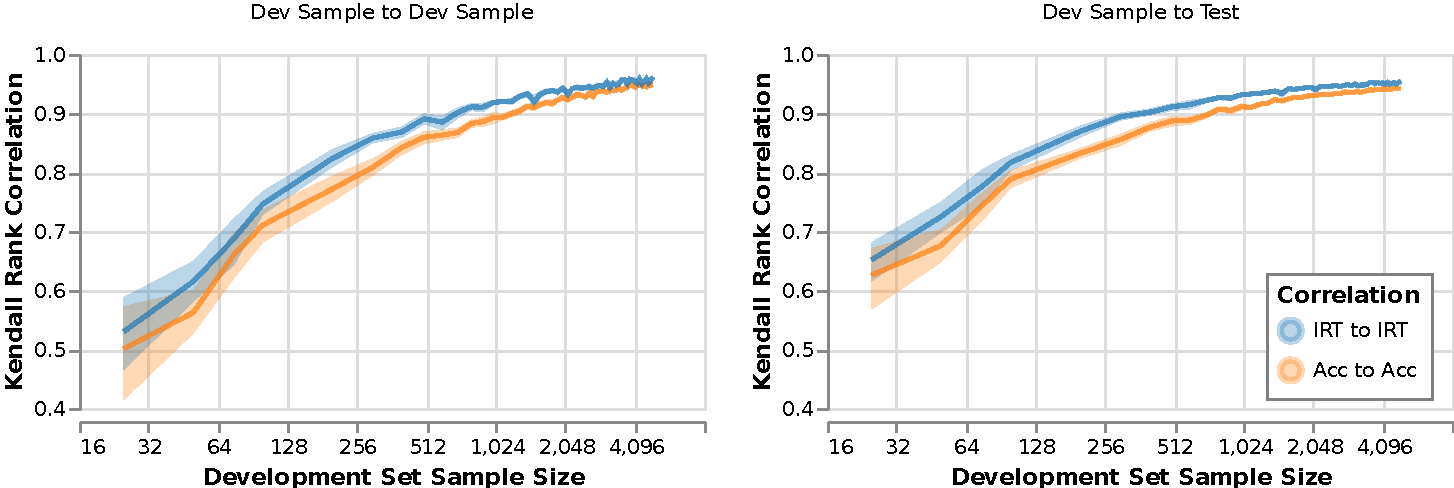
\includegraphics[width=\textwidth]{stability_simulation_corr}
    \caption{
        Compared to the final ranking over a large test set, how well does a small test set correlate?
        %
        The left shows correlation between mutually exclusive development set samples and the right between development samples and the full test set.
        %
        In both experiments (panes), ranking systems by \irt{} ability is more stable---across all sample sizes---than mean accuracy and thus more reliable (Kendall's rank correlation is higher).
        %
        Bands show 95\% confidence intervals of rank correlations across ten trials per sample size.
    }
    \label{fig:stability}
\end{figure*}

Rankings should be reliable within the same dataset (e.g., on dev
set) and generalize to similar datasets (e.g., with a test dataset).
%
To test the first, we measure the ranking stability of mutually
exclusive samples of the development
data~\cite{buckley2000measure}.
%
To test the second, we measure the correlation between
development set sample rankings to test set rankings~\citep{voorhees1998var}.

Specifically, for a range of sample sizes\footnote{ The sample size
    must be less than half the size of the development data so that we
    can obtain two samples.  } we (1) sample two partitions of the data,
(2) compute the classical ranking\footnote{For \squad{}, ordering by
    mean exact match score.} and the \irt{} ranking from a refit
\pl{3}~model, then (3) compute Kendall's
correlation~\citep{kendall1938tau} between the samples for each
ranking (details in Appendix~\ref{ch:isicle:apx:rank-stability}).
%
In both cases \irt{} rankings have higher correlation than classical
rankings (Figure~\ref{fig:stability}, left).
%
Since the benefit is strongest at low sample sizes, \irt{} can improve
the reliability of small-scale evaluations.
% Checking for ranking stability assesses the degree to which noise from data collection affects reliability, but does not address how good a predictor development performance is of test performance.

The second experiment examines ranking generalization: \irt{} yields more reliable measures of \subj{} skill,  implying a greater consistency in subject rankings across evaluation settings.
Figure~\ref{fig:stability} compares the development set sample rankings computed above to rankings obtained using subjects' \emph{test} set responses (with the same \irt{} model).

Across all sample sizes, subjects' \irt{} ability estimated on the
development set correlates well test set ability.
%
Crucially, this is better than the corresponding classical metrics
like accuracy (Appendix~\ref{ch:isicle:apx:rank-stability} quantifies
the statistical significance of the difference), supporting our
original motivation for using \irt{}.\footnote{ Since the maximum trial size was
    limited, we train one final model with the full data, see
    Table~\ref{tab:rank-corr} in the
    Appendix~\ref{ch:isicle:apx:rank-stability}.  }

\subsection{IRT Improves Cold Start Reliability}
\label{ch:isicle:sampling}

\irt{} can also guide the construction of tests.
Just as \irt{} practitioners prepare tests for humans, we too construct tests for machines.
In educational testing, collecting responses from humans is expensive; likewise, although \emph{questions} are cheap in search-based \qa{} tasks~\citep{Nguyen2016MSMA,kwiatkowski2019nq}, annotating \emph{answers} is expensive.
Likewise, ``grading'' machine dialog responses is expensive and \irt{} helps~\citep{sedoc2020irt}.
To emulate this setting, we use computerized adaptive testing~\citep{weiss1984cat} to iteratively select \squad{} \itms{} to ``annotate.''

As in human test preparation, we use existing annotations to infer
\itm{} parameters and iteratively infer the ability of new \subjs{}.
%
This experiment splits~$m$ \subjs{} into a training group (80\%) and a
testing group (20\%).
%
The training group represents \subjs{} for which we have full \itm{}
predictions and annotations; the testing group represents a new group
of \subjs{} that we need to rank.
To efficiently rank, we should iteratively choose \itms{} to annotate that yield the most information about the ranking if all the data were annotated.

This experiment compares how well several \itm{} selection strategies work.
For each selection method, we (1) choose a sample size, (2), sample
from the development set, (3) compute the ranking of \subjs{}, and (4)
compute Kendall's rank correlation
(Figure~\ref{fig:stability:sampling}).\footnote{We compute correlations with the complete development set on ten trials to build $95\%$ confidence intervals.}


\begin{figure}[t]
    \centering
    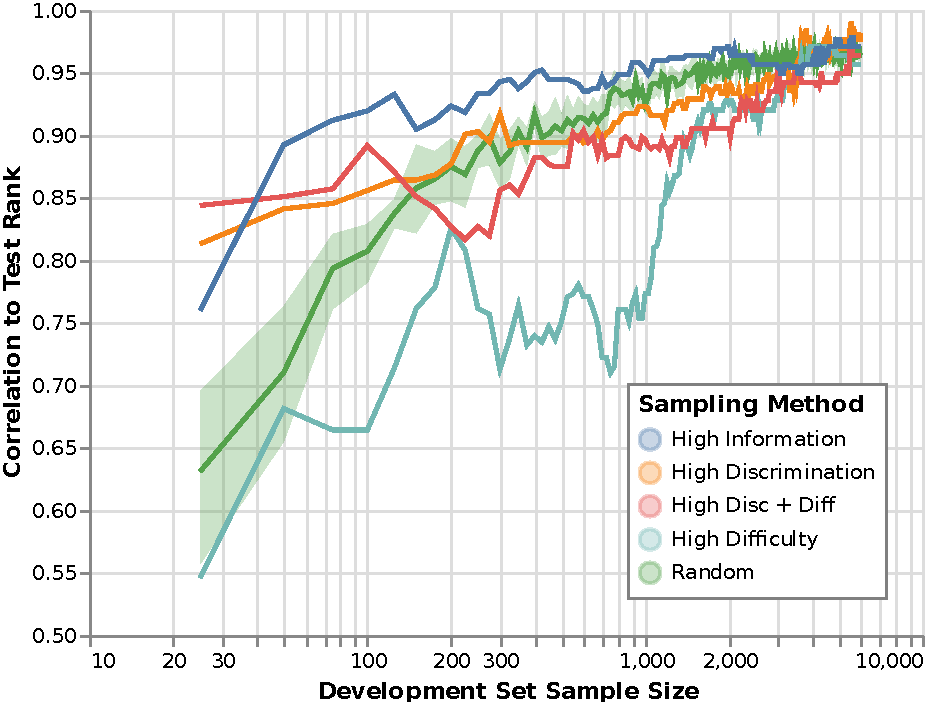
\includegraphics[width=\columnwidth]{cat_sampling_rank}
    \caption{
        Suppose we need to cold start and collect annotations for a new \subj{}: what order would most rapidly increase correlation to the full test data?
        As we expect, the correlations eventually converge, but with little data, \irt{} has better correlation than other methods.
        We suspect that the \irt{} information underperforms early on
        when the \subj{} ability estimate is unstable.
    }
    \label{fig:stability:sampling}
\end{figure}

% \jbgcomment{Below paragraph needs more intuition (both overall and for
%   the equation).  Currently, this is also stuck at the top of a page
%   in my compile, would be good to unpin it so that we don't have
%   widow.}

Which \itm{} selection strategies should we compare?
As a baseline, we use na\"ive random sampling.
Like prior work, we compare selecting \itms{} with the highest \diff{} and the highest \discability{}~\citep{lalor2019latent} as well as the sum of the two.\footnote{We train an \pl{2}~model to simplify sampling (e.g., avoiding a tradeoff between feasibility and \discability{}).}
We propose that \itms{} should be selected according to their Fisher information content~\citep{weiss1982info}
\begin{equation}
    \label{eq:info}
    I_i(\theta_j)=\frac{(p_{ij}')^2}{p_{ij}(1-p_{ij})}=\gamma_i^2 p_{ij}(1-p_{ij})
\end{equation} as derived by \citet[p. 70]{lord1968test}.

Intuitively, if we do not yet know the true skill~$\theta_j$, we should pick \itms{} whose expected response we are most uncertain about.
Our uncertainty (entropy) is maximized when the likelihood of a correct response $p_{ij}$ is the same as the likelihood of an incorrect response $1-p_{ij}$, which corresponds to the maximal value of $I_i(\theta_j)$; it is also sensible this value increases as \discability{} $\gamma_i$ increases.

To infer the maximally informative \itms{}, we estimate the ability
$\theta_j$ of each \subj{} using the currently selected \itms{}, use
the ability to compute the information
of each yet-to-be-annotated \itm{} for each \subj{}, and then aggregate the informativeness
\begin{equation}
    \text{Info}(i)=\sum_j I_i(\theta_j)
\end{equation}
by \itm{}~$i$ summed over \subjs{}~$j$.
This approach is similar to uncertainty sampling and reduces to it for the \pl{1}~model~\citep{lewis1994uncertainty}.
We initially seed with the twenty-five most discriminative \itms{} (details in Appendix~\ref{ch:isicle:apx:rank-stability}).

Like computerized adaptive testing~\citep{moreno1984cat}, Figure~\ref{fig:stability:sampling} shows that at lower sample sizes three of the \irt{} sampling methods are better than random sampling---\diff{} does worse.
The other \irt{} methods have comparable correlation.
Thus, by using \irt{}, \name{} can both improve rankings and guide annotation.
